\section{The modular group and continued fractions}

For an arbitrary modular transformation $A$, a representation as product of shifts $U^j: z \mapsto z+j$ and inversions $T: z \mapsto -\reci{z}$ can be found by the $T$-$U$ algorithm of Corollary \ref{cor_ModGrpTUAlg}. By writing out this product, for example in the case when $n=2$, we have
\begin{equation*}
A = U^{e_0}T U^{e_1}T U^{e_2}T U^k,
\end{equation*}
or more explicitly
\begin{equation}
\label{eqn_ALongConFrac}
A(z) = e_0 - \reci{e_1 - \reci{e_2 - \reci{k + z}}}.
\end{equation}
\index{Continued fraction}
\index{Pringsheim notation}
Here a close relation between modular transformations and continued fractions immediately gets apparent. In this section we will investigate this relation somewhat deeper. 
First we will use Pringsheim's more space-saving notation for continued fractions, namely
\begin{equation}
\label{eqn_ConFracNotation}
b_0 + \frac{a_1}{b_1 + \frac{a_2}{b_2 + \frac{a_3}{b_3 + \dots}}} =: 
b_0 + \cfr{a_1}{b_1} + \cfr{a_2}{b_2} + \cfr{a_2}{b_3} + \dots
\end{equation}
In the case when all $a_j = 1$, we adhere to the standard sequence notation for continued fractions:
\begin{equation*}
b_0 + \reci{b_1 + \reci{b_2 + \dots}} =: [b_0,b_1,b_2,\dots].
\end{equation*}
\index{Convergent}
For determining a continued fraction representation for a real number $\alpha$ such that all $a_j = 1$, one usually sets $\alpha_0 := \alpha$ as well as $b_j := \floor{\alpha_j}$ and $\alpha_{j+1} := \reci{\alpha_j - b_j}$ for $j \ge 0$ until some $\alpha_j$ is zero (which is the case if and only if $\alpha \in \Q$). In any way we obtain a finite or infinite sequence of equations 
\begin{equation}
\label{eqn_ConFracEqnSeq}
\alpha = \alpha_0 = b_0 + \reci{\alpha_1}, \quad
\alpha_1 = b_1 + \reci{\alpha_2}, \quad
\alpha_2 = b_2 + \reci{\alpha_3}, \quad \dots
\end{equation}
giving rise to the continued fraction representation $\alpha = [b_0, b_1, b_2, \dots]$. The rational number $c_n := [b_0,b_1,\dots,b_n]$ obtained by truncating the continued fraction representation after the coefficient $b_n$, is called the $n$-th \emph{convergent} of the continued fraction. If the continued fraction is infinte, \ie $\alpha \in \R \setminus \Q$, then we have $\lim_{n \to \infty} c_n = \alpha$.

\begin{remark}
\label{rem_ConFracKinds}
\index{Continued fraction!regular}
Note that by using the method above, all the coefficients $b_j$ with $j > 0$ are positive. A representation for $\alpha$ of this form is called a \emph{regular continued fraction} -- see also \Lehner{}, �9. 

\index{Continued fraction!semi-regular}
In contrast to that, if we set $b_j := \ceil{\alpha_j}$ for some or all of the indices $j$, then also negative coefficients $b_j$, $j > 0$, will occur and we obtain in this way a so called \emph{semi-regular continued fraction} representation of $\alpha$. This is in strong analogy to Remark~\ref{rem_EuclideanAlgorithmRounding} that within the Euclidean algorithm the quotients $q_j$ can be determined by rounding $r_{j-1} / r_j$ either up- or downward. Note that in \Lehner{}, �36, semi-regular continued fractions are defined such that for all $j > 0$ the coefficients $b_j$ are positive, but allowing for $a_j \in \{\pm 1\}$. However this makes no essential difference. 

\index{Continued fraction!canonical}
If we use the nearest integer function in each step, \ie $b_j := \nint{\alpha_j}$ for all $j$, then we have $\abs{b_j} \ge 2$ for all $j > 0$. If additionally $\alpha \in \Q$, then it can be shown that the resulting continued fraction representation is one of minimal length -- according to \Lehner{}, �39, we call finite continued fractions with this minimality property \emph{canonical continued fractions}.
\end{remark}

We can now reformulate Corollary \ref{cor_ModGrpTUAlg} in order to construct a continued fraction representation of any given modular transformation.

\begin{corollary}
\label{cor_ModTransConFrac}
An arbitrary modular transformation $A(z) = \moebius{a}{b}{c}{d}{z}$ can be written as continued fraction
\begin{equation}
\label{eqn_ModTransConFrac}
A(z) = [q_0,q_1,\dots,q_n,(-1)^{n+1}(k+z)]
\end{equation}
where the integers $n$, $q_0,q_1,\dots,q_n$ and $k$ are determined by the algorithm described in Corollary \ref{cor_ModGrpTUAlg}.
\end{corollary}
\begin{proof}
By using the continued fraction representation of $A$ given in (\ref{eqn_ALongConFrac}) and by applying the definition $e_j$ := $(-1)^j q_j$, we see
\begin{IEEEeqnarray}{rCcCcCcCcCcCc}
A(z) &=& e_0 &+& \cfr{-1}{e_1} 
          &+& \cfr{-1}{e_2} 
          &+& \dots 
          &+& \cfr{-1}{e_n} 
          &+& \cfr{-1}{k + z} \nonumber \\
  &=& q_0 &+& \cfr{-1}{-q_1} 
          &+& \cfr{-1}{q_2} 
          &+& \dots 
          &+& \cfr{-1}{(-1)^n q_n} 
          &+& \cfr{-1}{k + z}. \label{eqn_ModTransConFracInterim}
\end{IEEEeqnarray}
Now for every odd $j \le n$ we can rewrite 
\begin{equation*}
\cfr{-1}{-q_j} + \cfr{-1}{\dots} \quad \text{to} \quad \cfr{1}{q_j} + \cfr{1}{\dots}.
\end{equation*}
Thus if $n$ is odd, every numerator $-1$ in (\ref{eqn_ModTransConFracInterim}) can be turned into $+1$. In the other case, when $n$ is even, only one negative numerator at the end, $\frac{-1}{k+z}$, remains, but this can easily be rewritten to $\frac{1}{-(k+z)}$. Taking both cases together, we obtain (\ref{eqn_ModTransConFrac}).
\end{proof}

\begin{remark}
\label{rem_TUAlgConFrac}
It is worth noting that determining a continued fraction representation for a rational number $p/q \in \Q$ with $p,q \in \Z$ is essentially equivalent to applying the Euclidean algorithm to the integers $p$ and $q$: If we set $(r_{-1}, r_0) := (p,q)$ and substitute in (\ref{eqn_ConFracEqnSeq}) $\alpha_j = r_{j-1}/r_j$ for all $j \ge 0$, we obtain
\begin{IEEEeqnarray*}{rClCrCl}
\frac{r_{-1}}{r_0} &=& b_0 + \frac{r_1}{r_0} &\quad\Leftrightarrow\quad& 
  r_{-1} &=& b_0 \cdot r_0 + r_1 \\
\frac{r_0}{r_1} &=& b_1 + \frac{r_2}{r_1} &\Leftrightarrow& 
  r_0 &=& b_1 \cdot r_1 + r_2 \\
\frac{r_1}{r_2} &=& b_1 + \frac{r_3}{r_2} &\Leftrightarrow& 
  r_1 &=& b_2 \cdot r_2 + r_3 \\
 &\vdots& & & &\vdots&
\end{IEEEeqnarray*}
In other words, the coefficients $b_j$ of the desired continued fraction representation are nothing else but the quotients of the Euclidean algorithm which we used to denote by $q_j$.

This observation also allows it to see the $T$-$U$ algorithm of Corollary~\ref{cor_ModGrpTUAlg} in a different light: For a given modular transformation $A(z) = \moebius{a}{b}{c}{d}{z}$, by applying the Euclidean algorithm to $a$ and $c$, we effectively determine a continued fraction representation for the rational number $A(\infty) = \frac{a}{c} = [q_0,q_1,\dots,q_n]$. If we set again $e_j := (-1)^j q_j$, it follows that also the modular transformation $P := U^{e_0}T U^{e_1}T\dots U^{e_n}T$ maps $\infty$ to $\frac{a}{c}$. Since the stabilizer of $\infty$ is generated by the transformation $U$, all transformations with this property can be written as $PU^k$ for some $k \in \Z$.

In particular, if we determine the quotients $q_j$ by rounding to the nearest integer, we obtain a \emph{canonical continued fraction}, \ie a continued fraction representation of minimal length -- compare Remark~\ref{rem_ConFracKinds}. Consequently also the resulting $T$-$U$ product representation is one of minimal length.
\end{remark}

\begin{corollary}
\label{cor_ConFracModTrans}
Let $r \in \EQ$. A transformation $A \in \PSL{\Z}$ satisfying $A(\infty) = r$ can be found by determining a continued fraction representation of $r$, that is $r = [b_0,b_1,\dots,b_n]$, and setting $A := U^{e_0}T U^{e_1}T \dots U^{e_n}T$ where $e_j := (-1)^j b_j$. In particular, the $k$-th convergent $C_k$, $k \le n$, of this continued fraction representation can be written as $C_k = U^{e_0}T U^{e_1}T \dots U^{e_k}T(\infty)$.
\end{corollary}

We have now seen that there is a natural correspondence between rational numbers, continued fractions and the $T$-$U$ word representations of modular transformations. In order to formalize this correspondence, let us denote by $\Words{\Z} := \bigcup_{n \le 0} \Z^n$ the set of finite integer sequences (or words over the alphabet $\Z$). Furthermore we set $\EQ := \Q \cup \{\infty\}$ and define a map $f: \Words{\Z} \to \EQ$ by
\begin{equation}
\label{eqn_ConFracEvalMap}
\fundef{f}{\Words{\Z}}{\EQ}{(b_0,b_1,\dots,b_n)}{[b_0,b_1,\dots,b_n].}
\end{equation}
Note that evaluation of continued fractions shall take place in $\EQ$ with the natural conventions for treating infinite quantities, \ie for $a \ne 0$ and $b \ne \infty$ we have
\begin{equation*}
\frac{a}{0} = \infty,\quad \frac{b}{\infty} = 0,\quad b \pm \infty = \infty.
\end{equation*}
Moreover the empty continued fraction shall evaluate to $\infty$, \ie $f(\epsilon) = \infty$, where $\epsilon \in \Words{\Z}$ denotes the empty sequence. We call the sequence $\beta \in \Words{\Z}$ a \emph{continued fraction representation} for $f(\beta) \in \EQ$. %Two sequences $\beta, \gamma \in \Words{\Z}$ are defined to be \emph{equivalent}, in symbols $\beta \sim \gamma$, if and only if $f(\beta) = f(\gamma)$. 

Next we set $\Syms := \{T,U\} \subseteq \PSL{\Z}$ and let $\FreeGrp{\Syms}$ be the free group generated by the symbols $T$ and $U$. Moreover we denote by $\langle U \rangle$ both, the subgroup of $\FreeGrp{\Syms}$ generated by the symbol $U$ and the subgroup of $\PSL{\Z}$ generated by the transformation $U$. We now consider left cosets of $\langle U \rangle$ in  $\FreeGrp{\Syms}$ and $\PSL{\Z}$:
\begin{eqnarray*}
\FreeGrp{\Syms} / \langle U \rangle &:=& \setdef{\sigma \langle U \rangle}{\sigma \in \FreeGrp{\Syms}},\\
\PSL{\Z} / \langle U \rangle &:=& \setdef{A \langle U \rangle}{A \in \PSL{\Z}}.
\end{eqnarray*}
It is important to note these are \emph{not} factor groups, as $\langle U \rangle$ is not a normal subgroup of $\PSL{\Z}$ or $\FreeGrp{\Syms}$. In particular, neither $\PSL{\Z} / \langle U \rangle$ nor $\FreeGrp{\Syms} / \langle U \rangle$ carry a ``natural'' group structure -- we will regard them just as sets. 

We now have defined all domains needed for writing $f : \Words{\Z} \to \EQ$ as composition of three other functions, namely $f = g_3 \circ g_2 \circ g_1$, where
\begin{IEEEeqnarray*}{rCcCc}
g_1 &:& \Words{\Z} &\to& \FreeGrp{\Syms} / \langle U \rangle, \\
g_2 &:& \FreeGrp{\Syms} / \langle U \rangle &\to& \PSL{\Z} / \langle U \rangle, \\
g_3 &:& \PSL{\Z} / \langle U \rangle &\to& \EQ.
\end{IEEEeqnarray*}
Let us first turn to the definition of $g_1$, which maps a continued fraction representation to a left coset of a certain $T$-$U$ group word.
\begin{equation}
\label{eqn_MapConFracToPath}
\fundef{g_1}{\Words{\Z}}{\FreeGrp{\Syms} / \langle U \rangle}{(b_0,b_2,\dots,b_n)}{U^{e_0}T U^{e_1}T \dots U^{e_n}T \langle U \rangle} \quad \text{where } e_j := (-1)^j b_j.
%\fundef{g_1}{\Words{\Z}}{\FreeGrp{\Syms} / \langle U \rangle}{(b_0,b_2,\dots,b_n)}{\left( \prod_{j=0}^n (U^{e_j}T) \right) \langle U \rangle} \quad \text{where } e_j := (-1)^j b_j.
\end{equation}
Note that in the case of the empty sequence $\epsilon \in \Words{\Z}$ we have $g_1(\epsilon) = \langle U \rangle$.

In order to define $g_2$, let $\phi: \Sigma \to \PSL{\Z}$ be the canonical embedding, \ie $\phi(T) = T$ and $\phi(U) = U$. Let $\overline{\phi}$ be the unique extension of $\phi$ to a homomorphism $\FreeGrp{\Syms} \to \PSL{\Z}$, according to Theorem~\ref{thm_FreeGrpUniqueHom}. Note that $\overline{\phi}$ is just the map which evaluates $T$-$U$ group words to concrete elements of $\PSL{\Z}$ in the obvious way. The function $g_2$ now takes  a left coset in $\FreeGrp{\Syms}$ to a left coset in $\PSL{\Z}$ by
\begin{equation}
\label{eqn_MapPathToCoset}
\fundef{g_2}{\FreeGrp{\Syms} / \langle U \rangle}{\PSL{\Z} / \langle U \rangle}{\sigma \langle U \rangle}{\overline{\phi}(\sigma) \langle U \rangle.}
\end{equation}
Last but not least we define $g_3$ as the map which evaluates the transformations of a left coset $A \langle U \rangle \in \PSL{\Z} / \langle U \rangle$ at the point $\infty$. Note that the result is the same for all transformations within one coset because $\langle U \rangle$ is exactly the stabilizer of $\infty$, \ie $\langle U \rangle = \setdef{B \in \PSL{\Z}}{B(\infty) = \infty}$. This allows us to define
\begin{equation}
\label{eqn_MapCosetToEQ}
\fundef{g_3}{\PSL{\Z} / \langle U \rangle}{\EQ}{A \langle U \rangle}{A(\infty).}
\end{equation}

\begin{lemma}
\label{lem_ConFracMapEquality}
The maps $g_1$, $g_2$, $g_3$ and $f$, defined as above, satisfy
\begin{equation*}
f = g_3 \circ g_2 \circ g_1.
\end{equation*}
\end{lemma}
\begin{proof}
It follows from Corollary~\ref{cor_ConFracModTrans} that the composed map $g_2 \circ g_1: \Words{\Z} \to \PSL{\Z} / \langle U \rangle$ takes a continued fraction representation $(b_0,b_1,\dots,b_n)$ to a left coset $A \langle U \rangle$, such that $g_3(A \langle U \rangle) = A(\infty) = [b_0,b_1,\dots,b_n]$. Therefore we have indeed $f = g_3 \circ g_2 \circ g_1$.
\end{proof}

\begin{lemma}
\label{lem_MapConFracToPathInjective}
The map $g_1$ defined in (\ref{eqn_MapConFracToPath}) is injective. Its image $g_1(\Words{\Z})$ consists precisely of those cosets $\sigma \langle U \rangle \in \FreeGrp{\Syms} / \langle U \rangle$, where the $T$-$U$ group word $\sigma$ is such that:
\begin{enumerate}[\quad(i)]
\item \label{itm_NotContainsTInv}
The reduced form of $\sigma$ never contains the symbol $\inv{T}$.
\item \label{itm_RightmostIsT}
If the reduced form of $\sigma$ is not empty, its rightmost symbol is $T$.
\end{enumerate}
In particular there is a one-to-one correspondence between all continued fraction representations and $T$-$U$ group words of this form. 
\end{lemma}
\begin{proof}
The fact that $g_1$ is injective is obvious. It is also clear that the word
\begin{equation}
\label{eqn_ConFracTUWord}
U^{e_0}T U^{e_1}T \dots U^{e_n} T
\end{equation}
with $n \ge 0$, $e_j \in \Z$ occurring in the definition of $g_1$ already is in  reduced form and satisfies the conditions (\ref{itm_NotContainsTInv}) and (\ref{itm_RightmostIsT}). Conversely, every reduced word $w$ satisfying (\ref{itm_NotContainsTInv}) and (\ref{itm_RightmostIsT}) has necessarily the form
\begin{equation*}
w = U^{k_1} T^{\ell_1} U^{k_2} T^{\ell_2} \dots U^{k_m} T^{\ell_m},
\end{equation*}
with $m >= 0$, $k_j \in \Z$ and $\ell_j \ge 1$. Because for $k \ge 1$, $T^k$ and $(TU^0)^{k-1}T$ are \emph{identical} as words, we can for sure notate $w$ alternatively in the form (\ref{eqn_ConFracTUWord}).
\end{proof}

\begin{lemma}
\label{lem_MapCosetToEQBijective}
The map $g_3$ defined in (\ref{eqn_MapCosetToEQ}) is bijective. In particular there is a one-to-one correspondence between the left cosets of $\langle U \rangle$ in $\PSL{\Z}$ and the extended rational numbers $\EQ$.
\end{lemma}
\begin{proof}
If $g_3(A \langle U \rangle) = g_3(B \langle U \rangle)$, then $A(\infty) = B (\infty)$. This is equivalent to $\inv{B}A \in \langle U \rangle$ or $A \langle U \rangle = B \langle U \rangle$. Therefore $g_3$ is injective. Since $f = g_3 \circ g_2 \circ g_1$ is surjective, the same must be true for $g_3$.
\end{proof}

\begin{figure}
\centering
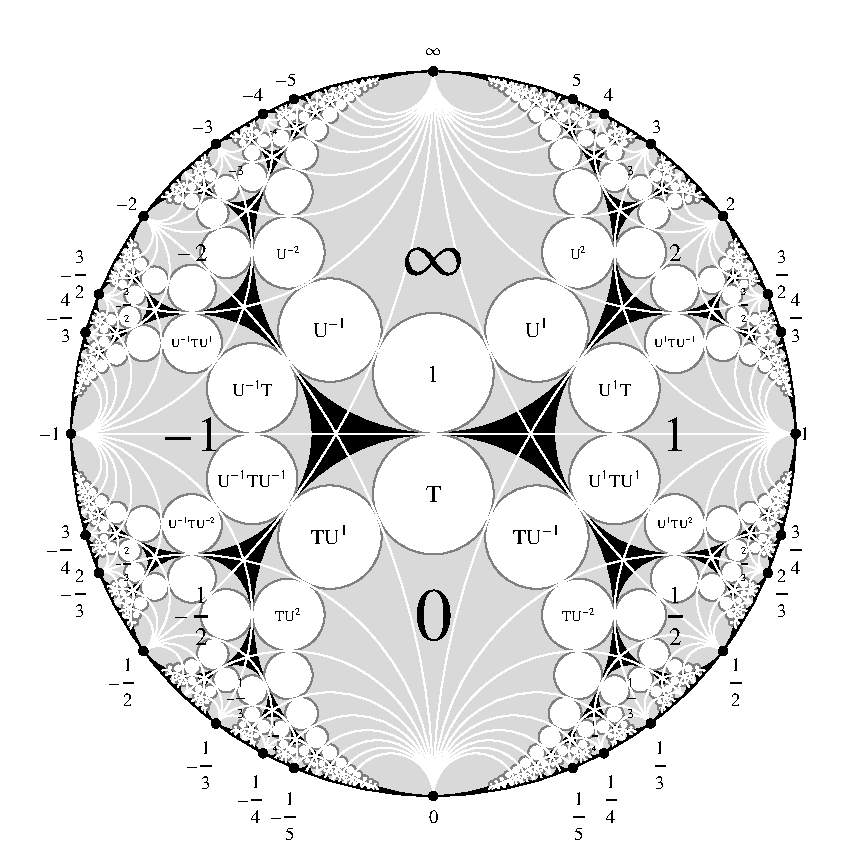
\includegraphics[width=\textwidth]{figures/ford-disks}
\caption{The modular tessellation under the modified Cayley transform $\ModCayley$. The Ford disk $\Forddisk_\infty$ (light gray, labeled with ``$\infty$'') encloses precisely the indisks $B\Indisk$, $B \in \langle U \rangle$, in its interior. It can thus be considered as representative for the subgroup $\langle U \rangle$ in $\PSL{\Z}$. The images of $\Forddisk_\infty$ under the modular group are all Ford disks $\Forddisk_r$ with $r \in \EQ$. For $A \in \PSL{\Z}$, we have $A\Forddisk_\infty = \Forddisk_r$ exactly when $A(\infty) = r$. Therefore $\Forddisk_r$ corresponds directly to both, the  number $r$ (the point, where $\Forddisk_r$ touches the extended real axis) and the left coset $A\langle U \rangle$ ($\Forddisk_r$ encloses precisely the indisks $B\Indisk$, $B \in A \langle U \rangle$).}
\label{fig_FordDisks}
\end{figure}
Looking at the modular tessellation, Figure~\ref{fig_ModularTiling}, we see that the images of the indisk $\Indisk$ of the fundamental region $\FunDom$ 
have a natural one-to-one correspondence to modular transformations, \ie the disk $A\Indisk$ can be considered as a graphical representative for the modular transformation $A$. The question arises, if there is such a visual and clear representation also for left cosets of $\langle U \rangle$ in $\PSL{\Z}$. Indeed, we can see in Figure~\ref{fig_FordDisks} -- depicting the modular tessellation under the modified Cayley transform $\ModCayley$ -- that the disks $U^k\Indisk$, $k \in \Z$ form a ``generalized ring'' which asymptotically approaches the point $\infty$. We can enclose this ring in a generalized disk -- in Figure~\ref{fig_FordDisks}, this enclosing disk is shown in light gray and is labeled with ``$\infty$''.
\begin{definition}
\label{dfn_FordDisk}
\index{Ford disk}
The unique (open) g-disk $\Forddisk_\infty$ containing all the disks $U^k\Indisk$, $k \in \Z$, in its interior and being tangent to each of them is called the \emph{Ford disk at $\infty$}. It contains all points $z \in \C$ with $\Im{z} > 1$. Its defining matrix is given by
\begin{equation}
\label{eqn_FordDisk}
\Forddisk_\infty : \mat{0}{-\ii}{\ii}{2}.
\end{equation}
For a modular transformation $A = \smallmat{a}{b}{c}{d} \in \PSL{\Z}$, the image of $\Forddisk_\infty$ under $A$ is called the \emph{Ford disk at $\frac{a}{c}$}, $\Forddisk_{\frac{a}{c}} := A\Forddisk_\infty$.
\end{definition}

The above definition as well as the bijective correspondence between left cosets of $\langle U \rangle$ in $\PSL{\Z}$ and the extended rational numbers $\EQ$ (Lemma~\ref{lem_MapCosetToEQBijective}) will get clearer in view of Figure~\ref{fig_FordDisks}: We can see that every Ford disk $\Forddisk_r$ (the light gray disks, each of them labeled with the corresponding number $r \in \EQ$), ``touches'' the extended real axis $\R_\infty := \R \cup \{\infty\}$ (appearing as unit circle under the modified Cayley transform) exactly in the point $r$, that is
\begin{equation*}
\topcl{\Forddisk_r} \cap \R_\infty = \{r\} \quad \text{for all } r \in \EQ.
\end{equation*}
For seeing the relation between Ford disks and left costets of $\langle U \rangle$ in $\PSL{\Z}$, first observe that the Ford disk $\Forddisk_\infty$ encloses precisely all indisks $B \Indisk$, $B \in \langle U \rangle$. In this sense, we can consider $\Forddisk_\infty$ as a graphical representative for the subgroup $\langle U \rangle$ of $\PSL{\Z}$. Every Ford disk $\Forddisk_r$, $r \in \EQ$, is the image of $\Forddisk_\infty$ under some transformation $A \in \PSL{\Z}$, \ie $A\Forddisk_\infty = \Forddisk_r$, which is the case if and only if $A(\infty) = r$. Consequently $\Forddisk_r$ encloses all indisks $B\Indisk$, $B \in A \langle U \rangle$ and thus can be considered as graphical representative for the coset $A \langle U \rangle$.

Also the statement of Lemma~\ref{lem_MapConFracToPathInjective}, the one-to-one correspondence between continued fraction representations and $T$-$U$ words of the form (\ref{eqn_ConFracTUWord}), has a nice visual interpretation, as we will illustrate in the following example.

\begin{figure}
\centering
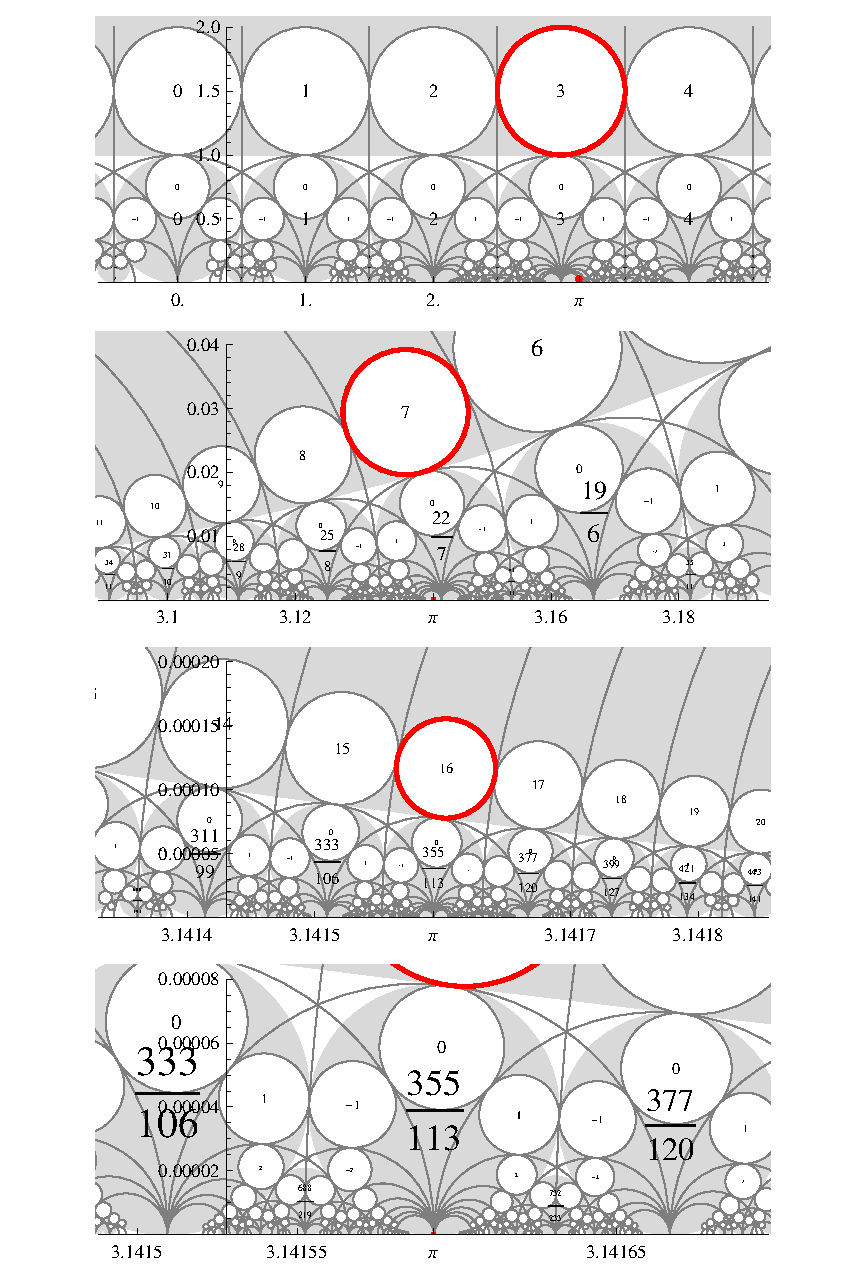
\includegraphics[width=\textwidth]{figures/cont-frac-pi}
\caption{$\pi = \frac{355}{113}$ -- well, almost.}
\label{fig_ConFracPi}
\end{figure}
\begin{example}
\label{ex_ConFracPi}
Consider the (semi-regular) continued fraction expansion of the irrational number $\pi$, obtained by using the nearest integer function for rounding the $\alpha_j$, as discussed in Remark~\ref{rem_ConFracKinds}. The first few coefficients of this continued fraction are given by
\begin{equation*}
\pi = [3, 7, 16, -294, 3, -4, 5, -15, -3, 2, 2, 2, 2, 3, -85, -3, 2, 15, 3, 14,\dots]
\end{equation*}
More coefficients can be found by looking up the sequence A133593 at the \emph{On-Line Encyclopedia of Integer Sequences (OEIS)}\footnote{https://oeis.org}. By Corollary~\ref{cor_ConFracModTrans}, the convergents of this continued fraction give rise to a sequence of Modular transformations:
\begin{IEEEeqnarray*}{rCcCl}
\lbrack 3 \rbrack &=& 3
  &=& U^3 T (\infty),\\
\lbrack 3,7 \rbrack &=& \frac{22}{7} 
  &=& U^3 T U^{-7} T (\infty),\\
\lbrack 3,7,16 \rbrack &=& \frac{355}{113}
  &=& U^3 T U^{-7} T U^{16} T (\infty),\\
\lbrack 3,7,16,-294 \rbrack &=& \frac{104348}{33215} 
  &=& U^3 T U^{-7} T U^{16} T U^{294} T (\infty),\\
&\vdots& &\vdots&
\end{IEEEeqnarray*}
The $T$-$U$ words occurring in this sequence can now be interpreted as ``path'' through the set of indisks $A\Indisk$, $A \in \PSL{\Z}$ as follows:
\begin{enumerate}
\item Start with the Ford disk $\Forddisk_\infty$. Label each indisk $U^k\Indisk$ (contained in $\Forddisk_\infty$) with the corresponding integer $k \in \Z$. The Ford disk $U^3 T \Forddisk_\infty = \Forddisk_3$, corresponding to the convergent $c_0 = 3$, can be approached by starting at the indisk $\Indisk$ (carrying the label 0), going 3 steps right to the indisk with label 3, $U^3 \Indisk$ (marked red in the first row of Figure~\ref{fig_ConFracPi}) and finally applying $T$, that is going from there to the tangent indisk $U^3 T \Indisk$, lying within the Ford disk $\Forddisk_3$.
\item For convenience, set $A_1 := U^3 T$. Within the Ford disk $\Forddisk_3$, label each indisk $A_1 U^k \Indisk$ with the \emph{negated}\footnote{The negation of the sign comes from the fact that we want the indisk labels to correspond to the coefficients $b_j$ of the continued fraction rather than to the exponents $e_j = (-1)^j b_j$ of the $T$-$U$ word.} integer $-k$. Go from indisk $A_1 \Indisk$ (labeled 0) seven steps to the indisk with label 7, $A_1 U^{-7}\Indisk$ -- see second row of Figure~\ref{fig_ConFracPi}. Applying $T$ again takes us to the indisk $A_1 U^{-7} T \Indisk$ within the Ford disk corresponding to the next convergent of the continued fraction: $\Forddisk_{c_1}$, $c_1 = \frac{22}{7}$.
\item Set $A_2 := U^3 T U^{-7} T$. As above, label all indisks $A_2 U^k \Indisk$ within $\Forddisk_{c_1}$ with $k$ and go from $A_2 \Indisk$ with label 0 sixteen steps to $A_2 U^{16} \Indisk$ with label 16 (Figure~\ref{fig_ConFracPi}, 3rd row) and from there to $A_2 U^{16} T \Indisk$, lying within $\Forddisk_{c_2}$, $c_2 = \frac{355}{113}$.

\dots
\end{enumerate}
\end{example}

Without explicating further steps of the above example, we can easily imagine how this generalizes to different continued fraction representations of arbitrary real numbers: Given a continued fraction $\alpha = [b_0,b_1,\dots]$, we start with the indisk $\Indisk^{(0)} := \Indisk$ contained in the Ford disk $\Forddisk^{(0)} := \Forddisk_\infty$. For every $j \ge 0$, we label the indisks contained in $\Forddisk^{(j)}$ with successive integers in counter-clockwise direction (if $j$ is even) or in clockwise direction (if $j$ is odd) in such a way that the disk $\Indisk^{(j)}$ carries the label 0. Now we choose $\Indisk^{(j+1)}$ as the unique indisk which is exterior to $\Forddisk^{(j)}$ and tangent to the disk with label $b_j$ (within $\Forddisk^{(j)}$). Moreover we choose as $\Forddisk^{(j+1)}$ the unique Ford disk containing $\Indisk^{(j+1)}$. 

\index{Indisk!path}
Considering also ``intermediate'' indisks (those with labels between 0 and $b_j$ within $\Forddisk^{(j)}$), we describe in this way an \emph{indisk path}, or in other words a chain of successively tangent disks, through the set of all indisks $A\Indisk$, $A \in \PSL{\Z}$. Such a path always starts at $\Indisk$ and, in case of a rational number $\alpha \in \EQ$, ends at some $U^{e_0}T U^{e_1}T \dots U^{e_n}T\Indisk$, appending exactly one symbol $U$, $\inv{U}$ or $T$ to the corresponding group word when moving one step forward along the path. Obviously these paths can be considered as a visual representation of $T$-$U$ words of the form (\ref{eqn_ConFracTUWord}) and we can draw the following conclusions:
\begin{corollary}
Continued fraction representations are not unique in any way.
\end{corollary}
\begin{proof}
All different indisk paths starting at $\Indisk$ and ending within a given Ford disk $\Forddisk_r$ give rise to different continued fraction representations for the same rational number $r \in \EQ$. Continued fraction representations are therefore not unique, unless we impose certain conditions on its coefficients $b_j$, as for example regularity -- compare \Lehner{}, �9.
\end{proof}
\begin{corollary}
Canonical continued fraction representations are in general not unique.
\end{corollary}
\begin{proof}
Considering a continued fraction representation $r = [b_0,b_1,\dots,b_n]$ of a rational number $r \in \EQ$, its length $n$ is exactly the number of hops between tangent Ford disks in the corresponding indisk path (or the number of symbols $T$ in the corresponding $T$-$U$ word). Let us call $n$ the \emph{length} of the indisk path. Note that Ford disks may possibly be visited more than once while walking along indisk paths. Clearly this is not the case if the path is one of minimal length from $\Forddisk_\infty$ to $\Forddisk_r$. Still, minimality with regard to path length does not imply uniqueness:  Consider for example $r = \frac{2}{5}$. In Figure~\ref{fig_FordDisks}, we can see $\Forddisk_{2/5}$ as the smaller of the two Ford disks being tangent to $\Forddisk_{1/3}$ and $\Forddisk_{1/2}$. We can see that there are three paths of length 3 from $\Forddisk_\infty$ to $\Forddisk_{2/5}$, namely
\begin{equation*}
\infty \to 0 \to \reci{2} \to \frac{2}{5},\quad
\infty \to 0 \to \reci{3} \to \frac{2}{5},\quad
\infty \to 1 \to \reci{2} \to \frac{2}{5}.
\end{equation*}
Since these paths are of minimal length, they give rise to three different  continued fraction representations of $r$ having minimal length:
\begin{equation*}
r = \frac{2}{5} = [0,2,2] = [0,3,-2] = [1,-2,3].\qedhere
\end{equation*}
\end{proof}

Considering indisk paths, we can also give an alternative proof for the following fact:
\begin{corollary}
All relations satisfied by the generators $T,U \in \PSL{\Z}$ are derived from $T^2 = 1$ and $(TU)^3 = 1$.
\end{corollary}
\begin{proof}
As above, in the definition of the map $g_2$ in (\ref{eqn_MapPathToCoset}), let again $\FreeGrp{\Syms} := \langle T, U \rangle$ be the free group of $T$-$U$ words, and let $\overline{\phi} : \FreeGrp{\Syms} \to \PSL{\Z}$ be the natural evaluation map. We need to show that every relation $\sigma \in \FreeGrp{\Syms}$ (satisfying $\overline{\phi}(\sigma) = 1$) can be written as product of words conjugate to $T^2$ and $(TU)^3$, that is
\begin{equation}
\label{eqn_RelationReduction}
\sigma = \prod_{j=1}^n (\tau_j R_j \inv{\tau_j})^{k_j},
\end{equation}
with $k_j \in \Z$, $\tau_j \in \FreeGrp{\Syms}$ and $R_j$ being either the word $T^2$ or $(TU)^3$. From $\overline{\phi}(\sigma) = 1$ we see that the indisk path corresponding to $\sigma$ is closed, \ie it starts and ends at the indisk $\Indisk$. Let us call such an indisk path a \emph{loop}. Next, set $\rho := \exp(2 \pi \ii / 3)$ and denote by $[\rho]_\sim$ the orbit of $\rho$ under $\PSL{\Z}$. We define the number of times a loop $L$ turns around a point $z \in [\rho]_\sim$ the \emph{winding number} $\nu_z(L)$. Every full turn around $z$ in positive (\resp negative) direction shall give a contribution of +1 (\resp -1) to $\nu_z(L) \in \Z$. If the winding number $\nu_z(L)$ is zero for all $z \in [\rho]_\sim$, we call $L$ a \emph{degenerate loop}. In this case $L$ consists enirely of subpaths of the form 
\begin{equation*}
\Indisk \to \Indisk_1 \to \dots \to \Indisk_{n-1} \to \Indisk_n \to \Indisk_{n-1} \to \dots \to \Indisk_1 \to \Indisk
\end{equation*}
and the corresponding $T$-$U$ word can be reduced to the empty word just by repeated application of the relation $T^2 = 1$. \index{Kronecker delta} Finally, using the \emph{Kronecker delta} notation,
\begin{equation*}
\delta_{z,w} := 
\begin{cases}
1 & \text{if } z = w,\\
0 & \text{otherwise,}
\end{cases}
\end{equation*}
we call a loop $L$ a \emph{primitive loop} for the point $z \in [\rho]_\sim$, if $\nu_w(L) = \delta_{w,z}$ for all $w \in [\rho]_\sim$. Looking at Figure~\ref{fig_FordDisks} and using its indisk labeling, the relation $(TU)^3 = 1$ corresponds to the loop
\begin{equation*}
L_\rho^\prime: 1 \to T \to TU \to \inv{U}T\inv{U} \to \inv{U}T \to \inv{U} \to 1.
\end{equation*}
We see that $L_\rho^\prime$ goes once around the point $\rho$ in clockwise (negative) direction. Going the loop in reverse direction yields a primitive loop for the point $\rho$, $L_\rho := \inv{(L_\rho^\prime)}$, corresponding to the relation $(TU)^{-3} = 1$. Next we define such a primitive loop $L_z$ for every $z \in [\rho]_\sim$. We do so by going from $\Indisk$ to any indisk in the ``neighbourhood'' of $z$ along a path $P_z$, then going around $z$ (and no other point) once in positive direction and finally returning to $\Indisk$ by going back the reverse path $\inv{P_z}$. Every such primitive loop $L_z$ corresponds to a relation of the form $\tau (TU)^{-3} \inv{\tau} = 1$.

Let now $\sigma \in \FreeGrp{\Syms}$ be an arbitrary relation, and call $S$ the closed indisk path corresponding to the word $\sigma$. There are only finitely many points $z \in [\rho]_\sim$ with $\nu_z(S) \ne 0$. We can therefore define a loop $V$ as the composition of primitive loops $L_z$, where $z$ runs over this finite set of points -- each primitive loop $L_z$ shall be taken as often as the winding number $\nu_z(S)$ declares:
\begin{equation*}
V := \prod_{z \in [\rho]_\sim} L_z^{\nu_z(S)}.
\end{equation*}
Note that the particular order of the individual factors in this product is irrelevant for our purposes. By going through the loop $S$ in forward and through $V$ in backward direction we obtain a degenerate loop $S\inv{V}$, \ie $\nu_z(S\inv{V}) = 0$ for all $z \in [\rho]_\sim$. In other words, with $V$ we have found a word $\psi \in \FreeGrp{\Syms}$ such that $\sigma\inv{\psi}$ can be reduced to 1 entirely by applying the relation $T^2 = 1$, \ie we have $\sigma\inv{\psi}\inv{\omega} = 1$ for some product $\omega \in \FreeGrp{\Syms}$ consisting entirely of factors conjugate to the word $T^2$. Therefore, with $\omega\psi$ we have found for the relation $\sigma$ a product representation of the desired form (\ref{eqn_RelationReduction}).
\end{proof}
